% The generic preamble
\documentclass[10pt,letterpaper,fleqn,titlepage]{article}

% Define packages to use
\usepackage{natbib}
\usepackage[dvips]{graphicx,color}
\usepackage{amsmath,amssymb}
\usepackage{bm}
\usepackage{caption}
\usepackage{xr}
\usepackage{ifthen}
\usepackage[dvipdfm,colorlinks,linkcolor=blue,citecolor=blue,urlcolor=blue]{hyperref}
\usepackage{fancybox}
\usepackage{textcomp}
\usepackage{alltt}
%\usepackage{floatflt}
%\usepackage{svn}


% Redefine default page
\setlength{\textheight}{9in}  % 1" above and below
\setlength{\textwidth}{6.75in}   % 0.5" left and right
\setlength{\oddsidemargin}{-0.25in}

% Redefine default paragraph
\setlength{\parindent}{0pt}
\setlength{\parskip}{1ex plus 0.5ex minus 0.2ex}

% Define caption width and default fonts
\setlength{\captionmargin}{0.5in}
\renewcommand{\captionfont}{\sffamily}
\renewcommand{\captionlabelfont}{\bfseries\sffamily}

% Define commands for super- and subscript in text mode
\newcommand{\superscript}[1]{\ensuremath{^\textrm{#1}}}
\newcommand{\subscript}[1]{\ensuremath{_\textrm{#1}}}

% Derived commands
\newcommand{\invcm}{\textrm{cm\superscript{-1}}}
\newcommand{\micron}{\ensuremath{\mu\textrm{m}}}

\newcommand{\df}{\ensuremath{\delta f}}
\newcommand{\Df}{\ensuremath{\Delta f}}
\newcommand{\dx}{\ensuremath{\delta x}}
\newcommand{\Dx}{\ensuremath{X_{max}}}
\newcommand{\Xeff}{\ensuremath{X_{eff}}}

\newcommand{\water}{\textrm{H\subscript{2}O}}
\newcommand{\carbondioxide}{\textrm{CO\subscript{2}}}
\newcommand{\ozone}{\textrm{O\subscript{3}}}

\newcommand{\taup}[1]{\ensuremath{\tau_{#1}}}
\newcommand{\efftaup}[1]{\ensuremath{\tau_{#1}^{*}}}

\newcommand{\textbfm}[1]{\boldmath\ensuremath{#1}\unboldmath}

\newcommand{\rb}[1]{\raisebox{1.5ex}[0pt]{#1}}

\newcommand{\f}[1]{\texttt{#1}}

% Define how equations are numbered
\numberwithin{equation}{section}
\numberwithin{figure}{section}
\numberwithin{table}{section}

% Define a command for title page author email footnote
\newcommand{\email}[1]
{%
  \renewcommand{\thefootnote}{\alph{footnote}}%
  \footnote{#1}
  \renewcommand{\thefootnote}{\arabic{footnote}}
}

% Define a command to print the Office Note subheading
\newcommand{\notesubheading}[1]
{%
  \ifthenelse{\equal{#1}{}}{}
  { {\Large\bfseries Office Note #1\par}%
    {\scriptsize \sc This is an unreviewed manuscript, primarily intended for informal}\\ 
    {\scriptsize \sc exchange of information among JCSDA researchers\par}%
  }
}

% Redefine the maketitle macro
\makeatletter
\def\docseries#1{\def\@docseries{#1}}
\def\docnumber#1{\def\@docnumber{#1}}
\renewcommand{\maketitle}
{%
  \thispagestyle{empty}
  \vspace*{1in}
  \begin{center}%
     \sffamily
     {\huge\bfseries Joint Center for Satellite Data Assimilation\par}%
     \notesubheading{\@docnumber}
  \end{center}
  \begin{flushleft}%
     \sffamily
     \vspace*{0.5in}
     {\Large\bfseries\ifthenelse{\equal{\@docseries}{}}{}{\@docseries: }\@title\par}%
     \medskip
     {\large\@author\par}%
     \medskip
     {\large\@date\par}%
     \bigskip\hrule\vspace*{2pc}%
  \end{flushleft}%
  \newpage
  \setcounter{footnote}{0}
}
\makeatother
\docseries{}
\docnumber{}


% Define a command for a DRAFT watermark
\usepackage{eso-pic}
\newcommand{\draftwatermark}
{
  \AddToShipoutPicture{%
    \definecolor{lightgray}{gray}{.85}
    \setlength{\unitlength}{1in}
    \put(2.5,3.5){%
      \rotatebox{45}{%
        \resizebox{4in}{1in}{%
          \textsf{\textcolor{lightgray}{DRAFT}}
        }
      }
    }
  }
}




% Define included documents
%\includeonly{}

% Title info
\title{Implementation of FASTEM4 in the CRTM}
\author{Paul van Delst\footnote{paul.vandelst@noaa.gov}\\JCSDA/EMC/IMSG\\[0.25in]
        David N. Groff\footnote{david.groff@noaa.gov}\\JCSDA/EMC/IMSG.}
\date{April, 2011}
\docnumber{??}

%-------------------------------------------------------------------------------
%                            Ze document begins...
%-------------------------------------------------------------------------------
\begin{document}
\maketitle

\draftwatermark

\section{Introduction}
This document describes the radiometric impact of implementing FASTEM4 on CRTM simulations.

\section{Radiometric Impact of FASTEM4 Implementation in the CRTM}
The radiometric impact of implementing FASTEM4 for any particular CRTM simulation depends on the channel central frequency, salinity, sea-surface temperature, surface wind speed and the angle between the wind direction and the sensor azimuth angle.  For a climatological tropical atmosphere we performed CRTM simulations using FASTEM4 and FASTEM1 for AMSUA NOAA-19, MHS NOAA-19, SSMIS F16 and AMSRE AQUA to assess how the magnitude of the radiometric impact depends on these inputs.  

\subsection{Dependance on Channel Frequency}
The channel central frequency determines the sensitivity to the surface and accounts for the most significant variability in the impact on CRTM simulations.  For example as shown in figure \ref{fig:AMSUA_Wind_Speed_Impact} the magnitude of the impact on NOAA-19 AMSUA simulations can vary from channel to channel by more than 5K.  With the exception of AMSRE Aqua channels 1-4 the CRTM simulations using FASTEM4 are colder for all the surface conditions we considered.  For AMSRE channels 1-4 the CRTM simulations using FASTEM4 can be 5K larger as shown in figure \ref{fig:AMSRE_Wind_Speed_Impact}.  Note that for AMSRE channels 1-6 the low frequency emissivity model was previously being used.

\begin{figure}[htp]
  \centering
  \includegraphics{graphics/AMSUA_Wind_Speed_BT.eps}
  \caption{The radiometric impact of implementing FASTEM4 on AMSUA NOAA-19 simulations as a function of wind speed.}
  \label{fig:AMSUA_Wind_Speed_Impact}
\end{figure}

\begin{figure}[htp]
  \centering
  \includegraphics{graphics/AMSRE_Wind_Speed_BT.eps}
  \caption{The radiometric impact of implementing FASTEM4 on AMSRE Aqua simulations as a function of wind speed.}
  \label{fig:AMSRE_Wind_Speed_Impact}
\end{figure}

\subsection{Dependence on Wind Speed}
The impact on CRTM simulations for microwave channels sensitive to the surface is most dependant on wind speed.  Figure \ref{fig:AMSUA_Wind_Speed_Impact} shows that the magnitude of the impact at wind speeds approaching 15 m/s are on the order of 2K larger than at wind speeds less than 4 m/s.  This result is corroborated by Figure \ref{fig:AMSUA_Background_Impact} which shows scatter plots of impact as brightness temperature differences for AMSUA metop-a using global NCEP background data from February 2, 2009 and August 1, 2009 as input.  

\begin{figure}[htp]
  \centering
  \includegraphics{graphics/AMSUA_Metop-a_Background.eps}
  \caption{The radiometric impact as a function of wind speed using global NCEP background data from February 2, 2009 and August 1, 2009 as input .}
  \label{fig:AMSUA_Wind_Speed_Impact}
\end{figure}

\subsection{Dependence on Salinity}
For AMSUA and MHS surface channels the impact decreases with increasing salinity as shown in figures \ref{fig:AMSUA_Salinity_Impact} and \ref{fig:MHS_Salinity_Impact}.  

\subsection{Dependence on the Angle Between the Sensor Azimuth and Wind Direction} 
The impact can vary significantly as a function of the angle between the sensor azimuth and wind direction.  The impact increases with the perpendicularity of the sensor azimuth to the wind direction.  When the sensor azimuths are perpedicular to the CRTM default wind direction of 0 degrees (or North) the magnitude of the brightness temperature differences are nearly 1K larger than those at sensor azimuths parallel or opposite to the wind direction as shown in figure \ref{fig:AMSUA_Sensor_Azimuth_Impact}.  
 

% The references section
%=======================
%\begin{thebibliography}{99}
%  \bibitem{ref:tag1} reference1
%  \bibitem{ref:tag2} reference2
%\end{thebibliography}

% The appendices section
%=======================
%\begin{appendix}
%\end{appendix}

\end{document}
